

\documentclass[10pt,twocolumn]{article}

% use the oxycomps style file
\usepackage{oxycomps}

% usage: \fixme[comments describing issue]{text to be fixed}
% define \fixme as not doing anything special
\newcommand{\fixme}[2][]{#2}
% overwrite it so it shows up as red
\renewcommand{\fixme}[2][]{\textcolor{red}{#2}}
% overwrite it again so related text shows as footnotes
%\renewcommand{\fixme}[2][]{\textcolor{red}{#2\footnote{#1}}}

% read references.bib for the bibtex data
\bibliography{references}

% include metadata in the generated pdf file
\pdfinfo{
    /Title (Predicting Solar Radiation using Machine Learning Techniques )
    /Author (Julia Chun)
}
\usepackage{tikz}
\usetikzlibrary{shapes.geometric, arrows}

% set the title and author information
\title{Comprehensive Project: {Solar Radiation Prediction Using Machine Learning}}
\author{Julia Chun}
\affiliation{Occidental College}
\email{jchun2@oxy.edu}

\begin{document}

\maketitle

\section{Problem Statement }
Climate change and global warming are global concerns where the implications are crucial and urgent. Changes to Earth's climate are driven by increased human emissions of greenhouse gases and these effects are seen having widespread effects on the environment. This concern is not a future problem as it was reported that effects that had long predicted would result from global climate change are now occurring, such as sea ice loss, accelerated sea level rise, and longer, more intense heat waves\cite{2}. Furthermore, these environmental implications impact various sectors of society and are interrelated. For instance, factors such as drought and flooding not only could cause damages to ecosystems and infrastructure, but could also impact food production and human health\cite{2}.

Solar radiation prediction plays a critical role in optimizing renewable energy systems and advancing climate science\cite{4}. This project focuses on predicting Global Horizontal Irradiance (GHI), an indicator of solar radiance, using machine learning techniques by leveraging data from the National Solar Radiation Database (NSRDB).  Accurate prediction of GHI is essential for optimizing solar energy systems, enhancing energy efficiency, and supporting the integration of renewable energy into the grid. However, modeling GHI is challenging due to the complex interplay of atmospheric conditions, geographic factors, and temporal variations.

This paper explores and compares different machine learning techniques—linear regression, decision trees, and stacking regressors—for modeling and predicting GHI at a given location. The primary goal is to assess the effectiveness of each technique in capturing the intricate patterns of solar radiation and providing reliable predictions.


\section{Technical Background}

\subsection{Key Solar Radiation Indicators in the Dataset}

The dataset utilized for this study contains several key solar radiation indicators that are fundamental to understanding and modeling solar energy systems. These indicators are essential for assessing the availability and variability of solar energy at a given location and are widely used in renewable energy research. Below is an explanation of the primary solar radiation indicators included in the dataset:

\subsubsection{Global Horizontal Irradiance (GHI)}
\begin{itemize}
     GHI represents the total solar radiation received per unit area on a horizontal surface\cite{7}. It is the sum of Direct Normal Irradiance (DNI) and Diffuse Horizontal Irradiance (DHI), adjusted for the angle of incidence of the sun.GHI is the most commonly used metric for photovoltaic (PV) systems, as it captures both direct and diffuse solar radiation\cite{7}. It provides a comprehensive measure of the total energy available for solar power generation on flat or slightly tilted surfaces. This feature could be usedin the design, performance assessment, and optimization of PV systems. It is also crucial for energy forecasting and resource assessment.
\end{itemize}

\subsubsection{Direct Normal Irradiance (DNI)}
\begin{itemize}
     DNI measures the amount of solar radiation received per unit area on a surface that is always perpendicular (normal) to the sun's rays. DNI accounts for only the direct beam of sunlight, excluding scattered or reflected radiation. It is highly sensitive to clear sky conditions and obstructions such as clouds or shading\cite{17}. This measure could be critical for concentrating solar power (CSP) systems, which rely exclusively on direct sunlight to generate energy\cite{17}. DNI is also used to calculate GHI and assess solar resource potential.
\end{itemize}

\subsubsection{Diffuse Horizontal Irradiance (DHI)}
\begin{itemize}
    DHI quantifies the portion of solar radiation that is scattered by the atmosphere and reaches the Earth's surface from all directions. It excludes the direct beam of sunlight. DHI becomes particularly important in cloudy or overcast conditions, where the contribution of direct sunlight is minimal\cite{17}. It reflects the impact of atmospheric conditions on solar radiation. This feature could be useful for designing systems in regions with high cloud cover or for understanding the contribution of diffuse light to overall energy generation\cite{17}.
\end{itemize}

\subsubsection{Global Normal Irradiance (GNI)}
\begin{itemize}
     GNI measures the total solar radiation received on a surface that is perpendicular to the sun’s rays. It is similar to DNI but includes the diffuse component when the surface is oriented directly toward the sun. GNI is useful for assessing the potential solar energy capture of surfaces that track the sun throughout the day. This feature can be relevant for solar tracking systems and for calculating energy yield in systems designed to maximize direct sunlight capture\cite{17}.
\end{itemize}

\subsubsection{Relationship Between Indicators}

These indicators are interrelated and together provide a complete picture of solar radiation at a given location:
\begin{itemize}
    \item \textbf{GHI} is calculated as:
    \[
    GHI = DNI \cdot \cos(\theta) + DHI
    \]
    where \( \theta \) is the solar zenith angle (the angle between the sun's rays and the vertical axis).
    \item \textbf{DNI} and \textbf{DHI} are independent components that reflect different aspects of solar radiation—direct and scattered light, respectively.
    \item \textbf{GNI} complements these by considering the orientation of the receiving surface relative to the sun.
\end{itemize}
\begin{figure}
    \centering
    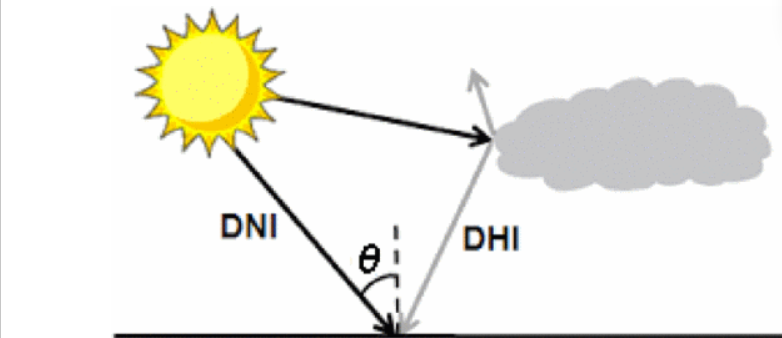
\includegraphics[width=1\linewidth]{GHI.png}
    \caption{Figure representing relationship between indicators.\cite{17}}
    \label{Figure 1}
\end{figure}

\subsubsection{Importance in Solar Energy Applications}

Understanding and utilizing these indicators can be essential for applications such as determining the suitability of different solar technologies (e.g., PV systems, CSP systems) for a given location or evaluating the energy yield and efficiency of solar installations under varying conditions. Furthermore, this could be useful when predicting solar energy availability to optimize grid integration and resource allocation.
\end{itemize}

\subsection{Machine Learning Models Used}

The project utilizes three machine learning models: linear regression, decision tree regression, and stacking regression. These models were chosen to explore the predictive capabilities of both simple and complex techniques for handling the relationships within the solar radiation dataset. Below is an explanation of each model:

\subsubsection{Linear Regression}
     Linear regression is a fundamental machine learning technique that models the relationship between a dependent variable (e.g., GHI) and one or more independent variables (e.g., temperature, cloud type) as a linear equation\cite{3}. The strength of a linear regression model is how it is interpretable, computationally efficient, and works well for features with strong linear relationships to the target variable\cite{3}. However, there are limitaions of a linear regression model as it struggles with capturing nonlinear relationships, which are common in solar radiation data due to factors like atmospheric scattering and cloud cover.


\subsubsection{Decision Tree Regression}
A decision tree regression is a non-linear model that splits the dataset into subsets based on feature values, forming a tree structure. Each split aims to minimize the variance within the resulting subsets.\cite{21} Decision trees can capture complex, nonlinear relationships and interactions between features. They are also interpretable, as the splits provide insight into the importance of features. Decision trees are prone to overfitting, especially with deep trees or when noise is present in the data.\cite{21}
\end{itemize}

\subsubsection{Stacking Regression}
A stacking regression is an ensemble learning technique that combines the predictions of multiple models (e.g., linear regression and decision tree) to produce a final prediction.\cite{22} The combined model, or meta-model, learns how to weight the contributions of the base models.Stacking can capture both linear and nonlinear relationships by leveraging the complementary strengths of different models.\cite{22} It often achieves higher accuracy than individual models. 
\end{itemize}

\subsubsection{Comparison and Rationale for Selection}
\begin{itemize}
    \item \textbf{Linear Regression:} Selected for its simplicity and interpretability, serving as a baseline for comparison with more complex models.
    \item \textbf{Decision Tree Regression:} Included for its ability to handle nonlinear dependencies and provide insights into feature importance.
    \item \textbf{Stacking Regression:} Chosen for its capacity to integrate multiple models, addressing both linear and nonlinear patterns for enhanced predictive performance.
\end{itemize}

By employing these models, the study aims to assess the effectiveness of different machine learning approaches in predicting solar radiation, offering insights into their strengths, limitations, and applicability to renewable energy systems.
\section{Evaluation Metrics for Model Evaluation}
The section discusses the metrics used for the evaluation of the machine learning models.

\begin{itemize}
    \item \textbf{Mean Absolute Error (MAE):}
    \begin{itemize}
        \item MAE calculates the average magnitude of errors between the predicted and actual values, providing an intuitive measure of accuracy without considering error direction. It is defined as:
        \[
        MAE = \frac{1}{n} \sum_{i=1}^n |y_i - \hat{y}_i|,
        \]
        where \( y_i \) represents actual values and \( \hat{y}_i \) represents predicted values.\cite{20}
    \end{itemize}

    \item \textbf{Root Mean Squared Error (RMSE):}
    \begin{itemize}
        \item RMSE measures the square root of the average squared differences between predicted and actual values, placing greater emphasis on larger errors.\cite{20} It is calculated as:
        \[
        RMSE = \sqrt{\frac{1}{n} \sum_{i=1}^n (y_i - \hat{y}_i)^2}.
        \]
    \end{itemize}

    \item \textbf{R-squared (\( R^2 \)):}
    \begin{itemize}
        \item  \( R^2 \) quantifies the proportion of variance in the target variable explained by the model.\cite{20} It is expressed as:
        \[
        R^2 = 1 - \frac{\sum_{i=1}^n (y_i - \hat{y}_i)^2}{\sum_{i=1}^n (y_i - \bar{y})^2},
        \]
        where \( \bar{y} \) is the mean of actual values.
    \end{itemize}

    \item \textbf{Predicted R-squared (Cross-Validation):}
    \begin{itemize}
        \item  Predicted \( R^2 \) evaluates the model's ability to generalize by computing \( R^2 \) using cross-validation. It indicates how well the model performs on unseen data.\cite{20}
    \end{itemize}
\begin{itemize}
    \item \textbf{Mean Absolute Percentage Error (MAPE):}
    \begin{itemize}
        \item  MAPE measures the average percentage difference between predicted and actual values.\cite{20} It is calculated as:
        \[
        MAPE = \frac{1}{n} \sum_{i=1}^n \left| \frac{y_i - \hat{y}_i}{y_i} \right| \times 100,
        \]
        where \( y_i \) represents actual values and \( \hat{y}_i \) represents predicted values.
    \end{itemize}

    \item \textbf{Adjusted R-squared:}
    \begin{itemize}
        \item  Adjusted \( R^2 \) modifies the \( R^2 \) value to account for the number of predictors in the model, penalizing unnecessary complexity.\cite{20} It is expressed as:
        \[
        \text{Adjusted } R^2 = 1 - \frac{(1 - R^2)(n - 1)}{n - p - 1},
        \]
        where \( n \) is the number of observations, \( p \) is the number of predictors, and \( R^2 \) is the unadjusted coefficient of determination.
    \end{itemize}

    \item \textbf{Normalized Metrics:}
    \begin{itemize}
        \item  Normalized versions of MAE and RMSE are calculated by dividing these values by the range of the target variable, providing a relative measure of error\cite{20}:
        \[
        \text{Normalized MAE} = \frac{MAE}{\text{max}(y) - \text{min}(y)}, \quad \text{Normalized RMSE} = \frac{RMSE}{\text{max}(y) - \text{min}(y)}.
        \]
    \end{itemize}
\end{itemize}


\section{Literature Review}

Accurate prediction of solar radiation, particularly Global Horizontal Irradiance (GHI), is critical for optimizing solar energy systems and supporting the integration of renewable energy into the grid. Several machine learning (ML) techniques, including linear regression, decision trees, and stacking regressors, have been explored to enhance predictive accuracy. Additionally, the selection of relevant features and the target variable plays a pivotal role in improving model performance. This section reviews relevant research, discusses the implications of feature and target variable selection, and highlights how these studies influenced the direction of this project.

\subsection{Linear Regression, Decision Trees, and Stacking Regressors in Solar Radiation Prediction}
Linear regression, being a simple and interpretable model, serves as a baseline for predictive tasks. However, it is limited to capturing linear relationships. Decision trees, on the other hand, can model complex, nonlinear interactions and hierarchical patterns in the data. Combining these models using stacking regressors has shown promise in leveraging the strengths of both techniques. Stacking regressors use a meta-learner, often linear regression, to aggregate predictions from base models, thereby improving accuracy and robustness.

Kumari and Toshniwal \cite{14} evaluated linear regression, decision trees, and other ML techniques for GHI prediction across 21 cities in India. Their results demonstrated that decision trees and ensemble models significantly outperformed linear regression, particularly for datasets exhibiting nonlinear patterns. Furthermore, random forest, a closely related ensemble technique, consistently provided higher predictive accuracy, emphasizing the potential of combining multiple models for solar radiation prediction. This inspired the inclusion of stacking regressors in this project, combining the simplicity of linear regression with the robustness of decision trees to achieve better predictions.

\subsection{Feature Selection and Its Importance}
Feature selection is a critical step in building accurate and efficient models. Including irrelevant or redundant features can lead to overfitting, increased computational complexity, and reduced interpretability. Studies like 'Effect of Feature Selection on the Prediction of
Direct Normal Irradiance' \cite{4} and 'Composition of feature selection techniques for improving the global horizontal irradiance estimation via machine learning models' highlight the importance of selecting impactful features.\cite{17} In 'Composition of feature selection techniques for improving the global horizontal irradiance estimation via machine learning models', features such as  Direct Normal Irradiance (DNI) and Diffuse Horizontal Irradiance (DHI), Clearsky DNI, Clearsky DHI, Solar Zenith Angle, and Temperature were found to be the most impactful features\cite{17}. By using tree-based models like random forest and XGBoost to assess feature importance, they demonstrated that focusing on key predictors enhances both prediction accuracy and computational efficiency. However, features such as DNI, DHI, Clearsky DNI, and Clearsky DHI would be decided to be dropped from my dataset/study as they are other measures of solar radiation. The paper 'Solar irradiance forecasting models using machine learning techniques and digital twin: A case study with comparison' found features such as temperature, cloudiness index, relative humidity, and day of the week were the most critical factors in predicting solar irradiance. The features temperature and solar zenith angle were consistently seen as highly correlated features to solar radiation in various studies.

This project was influenced by these findings to prioritize feature selection. The use of feature importance rankings from decision trees ensured that only the most relevant meteorological and temporal features were included, optimizing both model performance and interpretability.

\subsection{Target Variable: Global Horizontal Irradiance (GHI)}
GHI is the most commonly used target variable in solar radiation prediction due to its direct relevance to solar energy applications. Representing the total solar radiation received on a horizontal surface, GHI serves as a key input for designing and optimizing photovoltaic systems. Accurate GHI prediction is essential for estimating solar energy potential, improving energy efficiency, and supporting grid integration of solar power.

The paper 'Global Horizontal Irradiance' \cite{8}, emphasize that GHI prediction benefits from ensemble models that leverage diverse features and data sources. GHI's dependence on meteorological and temporal variables necessitates incorporating these factors into predictive models to capture its inherent variability. This insight guided the focus on GHI as the primary target variable in this project, ensuring alignment with real-world solar energy applications.

\subsection{Pearson Correlation Matrix}
The Pearson correlation matrix is a statistical tool used to measure the linear correlation between features and the target variable, GHI. It is particularly valuable for identifying which features have the strongest relationships with GHI, aiding in feature selection. Studies such as those by Boutahir et al. \cite{5} demonstrate the effectiveness of correlation analysis in filtering out irrelevant or redundant features. High correlation values indicate strong predictive potential, while low or near-zero values suggest limited relevance. The correlation matrix thus serves as a foundation for feature selection, ensuring that only impactful variables are included in the modeling process.

This project leveraged the Pearson correlation matrix to identify the top features influencing GHI, such as temperature, solar zenith angle, and relative humidity. By focusing on these variables, the models achieved improved interpretability and performance.

\subsection{Evaluation Metrics}
Evaluation metrics are essential for assessing the performance of predictive models and ensuring they meet project objectives. Metrics such as Mean Absolute Error (MAE), Root Mean Squared Error (RMSE), and \( R^2 \) score are widely used in solar radiation prediction studies. For example, Kumari and Toshniwal \cite{14} highlighted the importance of RMSE for quantifying prediction errors, while Boutahir et al. \cite{Boutahir2022} emphasized \( R^2 \) for measuring the goodness of fit. The consistent use of these metrics ensured meaningful comparisons across different models and datasets, guiding the evaluation and optimization processes.
\subsection{Ethical Considerations Literature}

Ethical considerations are pivotal in the development of climate technologies like Solar Radiation Management (SRM) and solar radiation prediction models. SRM, as discussed by Svoboda, involves reflecting solar radiation back into space to mitigate global warming \cite{11}. While promising, it raises concerns of moral hazard, procedural injustice, and intergenerational burdens. For example, unilateral deployment could marginalize vulnerable populations and create dependency for future generations.




By leveraging linear regression, decision trees, and stacking regressors, along with robust feature and target variable selection techniques, this study aims to advance the field of solar radiation modeling. These approaches ensure accurat and interpretable  predictions of GHI, facilitating the development of sustainable energy solutions. Insights from the literature not only guided the choice of models but also informed the importance of feature selection and the use of GHI as the target variable, ensuring the project's alignment with best practices in solar radiation prediction.

\bibliographystyle{unsrt}
\bibliography{references}



\section{Methods}

The methodology involved data collection, target variable selection, data preprocessing, feature selection, model selection, model training, and evaluation to systematically analyze and predict Global Horizontal Irradiance (GHI) using various modeling techniques. The approach was carefully designed, justified with respect to prior literature, and supported by intermediate decisions aimed at achieving robust predictions.

\subsection{Data Acquisition} 
\subsubsection{Database}
The datasets utilized for this study were sourced from the National Solar Radiation Database (NSRDB), a comprehensive resource maintained by the National Renewable Energy Laboratory (NREL). The NSRDB provides high-resolution solar radiation data, which is widely recognized and employed in renewable energy projects and academic research\cite{1}. The dataset's accessibility and proven reliability ensured compliance with ethical standards and compatibility with prior work.

\subsubsection{Dataset Content}
The datasets were extracted for predefined geographic locations based on latitude and longitude coordinates. Each dataset included consistent features and was retrieved for a specified year to ensure temporal alignment. The datasets encompassed 27 features spanning meteorological, atmospheric, solar radiation, cloud-related, and temporal variables. Key features included Global Horizontal Irradiance (GHI), Direct Normal Irradiance (DNI), Diffuse Horizontal Irradiance (DHI), air temperature, relative humidity, wind speed, atmospheric pressure, and cloud cover. Temporal features such as hour, day, and month added granularity.

The inclusion of variables aligned with prior literature, ensuring that the dataset captured critical factors influencing solar radiation. This alignment facilitated meaningful comparisons with established methodologies while providing a robust foundation for predictive modeling.

\subsection{Target Variable Selection}
The target variable selection process focused on identifying GHI as the primary metric for prediction, in comparison to other solar radiation indicators such as DNI, DHI, and Global Normal Irradiance (GNI). GHI's comprehensive nature, capturing both direct and diffuse solar radiation, made it the most practical and widely applicable measure for photovoltaic (PV) systems, which typically operate on flat or slightly tilted surfaces\cite{6}. Additionally, GHI's frequent use in prior studies highlighted its relevance and ensured alignment with existing research. By selecting GHI, this study aimed to maximize the practical utility and generalizability of the predictive models.

\subsection{Feature Exploration}
Initial feature exploration examined the relationships between the predictors and GHI using scatter plots, correlation matrices, and visual analytics. This step informed model selection by identifying linear and nonlinear dependencies in the data.

\subsubsection{Linear Relationships}
Features with predominantly linear relationships included:
\begin{itemize}
    \item \textbf{Temperature}: A positive linear trend, indicating that GHI increases with rising temperature.
    \item \textbf{Hour of the Day}: Predictable linear variations aligned with the diurnal solar cycle.
\end{itemize}

\subsubsection{Nonlinear Relationships}
Nonlinear relationships highlighted the complexity of the dataset, necessitating models capable of capturing such patterns:
\begin{itemize}
    \item \textbf{Cloud Type}: Variations in cloud type significantly affected GHI.
    \item \textbf{Solar Zenith Angle}: GHI peaked at small zenith angles and decreased nonlinearly as the angle increased.
    \item \textbf{Relative Humidity}: Threshold effects showed significant reductions in GHI at high humidity levels.
\end{itemize}

\subsection{Model Selection}
Three predictive models were chosen to address the identified linear and nonlinear relationships:
\begin{itemize}
    \item \textbf{Linear Regression}: Simple and interpretable, suitable for features with linear trends.
    \item \textbf{Decision Tree Regressor}: Captured nonlinear dependencies effectively.
    \item \textbf{Stacking Regressor}: Combined the strengths of both linear regression and decision trees to enhance accuracy and robustness.
\end{itemize}
The selection was guided by insights from feature exploration and prior literature, ensuring that the models addressed the complexities of the dataset while providing interpretable and scalable solutions.

\subsection{Feature Selection}
Feature selection aimed to retain the most impactful predictors while minimizing redundancy. A correlation matrix identified features with strong relationships to GHI, flagging variables with a correlation threshold above 0.07 as significant. The top features included Temperature, Hour, Solar Zenith Angle, Relative Humidity, and Cloud Type. Highly correlated features, such as temporal indicators (e.g., year, month, day). The result of the features temperature and solar zenith angle having high correlation to GHI is consistent with prior studies \cite{5},\cite{14},\cite{18}. Redundant solar radiation metrics (Clearsky GHI, Clearsky DHI, Clearsky DNI), were removed to avoid multicollinearity. This step streamlined the dataset to 16 features, enhancing interpretability and reducing computational complexity.
\begin{figure}
    \centering
    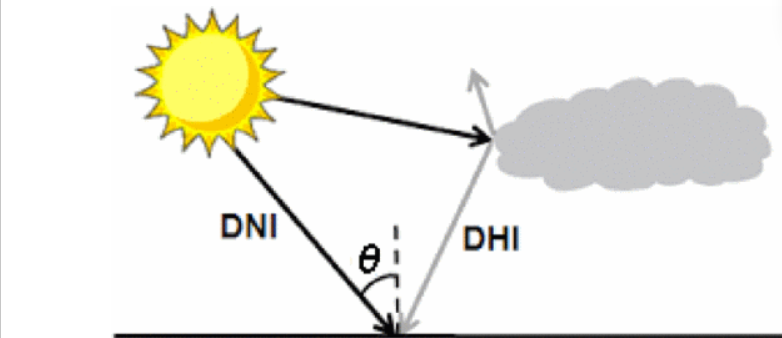
\includegraphics[width=0.5\linewidth]{GHI.png}
    \caption{Enter Caption}
\end{figure}
\begin{figure}
    \centering
    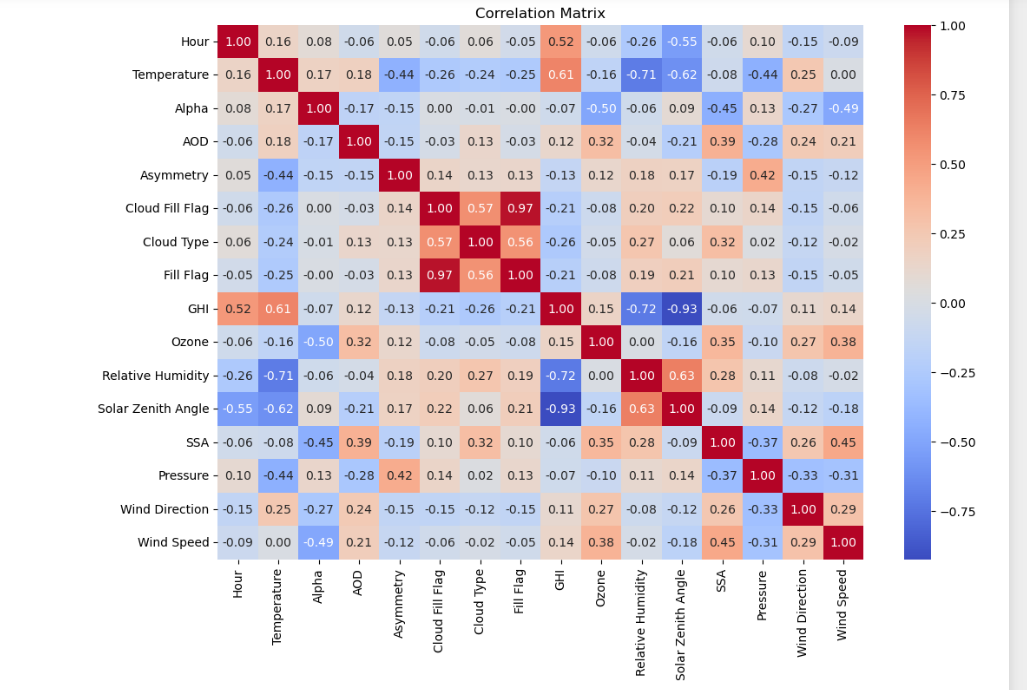
\includegraphics[width=1\linewidth]{fincorr.png}
    \caption{Final correlation matrix with reduced features.}
    \label{Figure 1}
\end{figure}

\subsection{Data Preprocessing}
Data preprocessing ensured the dataset's suitability for modeling. Cleaning steps addressed inconsistencies and errors, while feature engineering was deemed unnecessary due to the dataset's structured and complete nature. Missing values were already addressed within the NSRDB data collection framework, allowing a focus on feature reduction and preparation for model training.

\subsection{Model Training}
Models were trained using an 80-20 train-test split, balancing the need for sufficient training data with robust evaluation. This allocation aligned with best practices in machine learning literature, ensuring that the models had adequate exposure to the data for learning while reserving enough samples for independent testing.

\subsection{Hyperparameter Tuning}
To optimize model performance, hyperparameter tuning was performed, particularly for the decision tree regressor. A grid search technique evaluated combinations of parameters, such as maximum depth, minimum samples per split, and minimum samples per leaf. Cross-validation ensured that the selected parameters generalized well to unseen data, enhancing the model's reliability and accuracy.

\subsection{Alternate Approaches}
Alternate approaches, such as using deep learning models or unsupervised feature selection techniques, were considered but deemed outside the scope of this study due to computational complexity and data constraints. However, these approaches remain promising for future work, particularly in scenarios requiring real-time prediction or adaptation to larger datasets.

This structured methodology, supported by intermediate decisions and justified by prior work, ensured that the project's goals were met while maintaining alignment with the literature and addressing the complexities of solar radiation prediction.




\section*{Evaluation Metrics}

Evaluating the performance of machine learning models is essential to determine how well they address the problem of solar radiation prediction. This section describes the metrics used, their justification based on the literature and problem context, and discusses other potential metrics that were not included.

\subsection*{Metrics Used and Justification}

The following metrics were selected to evaluate the models. Furthermore, it was observed these metrics were widely used in solar radiation studies to evaluate prediction accuracy, as highlighted in prior literature \cite{4}\cite{3}\cite{5}.
\begin{itemize}
    \item \textbf{Mean Absolute Error (MAE):}
    \begin{itemize}
        \item This metric was used as it provides an intuitive measure of model accuracy by quantifying how far, on average, the predictions are from the actual values. 
    \end{itemize}

    \item \textbf{Root Mean Squared Error (RMSE):}
    \begin{itemize}
        \item  RMSE is particularly useful in scenarios where large prediction errors need to be penalized. In this project's prediction of GHI, it would help capture extreme deviations due to factors like unpredictable atmospheric conditions.
    \end{itemize}

    \item \textbf{R-squared (\( R^2 \)):}
    \begin{itemize}
        \item \textbf \( R^2 \) is a standard metric in regression analysis and provides an overall measure of model fit. High \( R^2 \) values would indicate that the model captures the variability in GHI effectively.
    \end{itemize}

    \item \textbf{Predicted R-squared (Cross-Validation):}
    \begin{itemize}
        \item \Generalizability is critical for solar radiation models, especially when applying them to different geographic regions. Using the predicted \( R^2 \) would ensure that the model is robust across varied datasets.
    \end{itemize}
\end{itemize}

\subsection*{Other Metrics and Their Exclusion}

While other metrics could have been used, their exclusion is justified as follows:
\begin{itemize}
    \item \textbf{Mean Absolute Percentage Error (MAPE):}
    \begin{itemize}
        \item MAPE measures errors as a percentage of actual values. However, it tends to inflate errors when actual values are near zero, making it less suitable for solar radiation datasets with varying magnitudes.
    \end{itemize}

    \item \textbf{Adjusted R-squared:}
    \begin{itemize}
        \item Adjusted \( R^2 \) accounts for the number of predictors in the model, penalizing unnecessary complexity. While useful, it was not prioritized as the models used are inherently simple or based on ensemble techniques.
    \end{itemize}

    \item \textbf{Normalized Metrics:}
    \begin{itemize}
        \item Normalized versions of MAE and RMSE (e.g., dividing by the range of the target variable) were excluded due to the limited benefit in interpretability for this specific problem.
    \end{itemize}
\end{itemize}

\subsection*{Conclusion on Metric Selection}

The selected metrics—MAE, RMSE, \( R^2 \), and predicted \( R^2 \)—offer a comprehensive evaluation framework for solar radiation prediction models. These metrics align with the problem's requirements by focusing on both accuracy and generalizability, and their selection is supported by existing literature. Future work could explore additional metrics, such as MAPE or adjusted \( R^2 \), if specific aspects like proportional errors or model complexity require emphasis.


A detailed comparison of these metrics across the three models would quantify their relative effectiveness in predicting GHI. For instance, while the linear regression model provides interpretability, its lower R\textsuperscript{2} score could highlight the limitations of linear assumptions.
\section{Case Studies}

Using the presented methodology, the following case studies were explored:

\subsection{Case Study 1: Model Performance on San Francisco Dataset (2022)}
The first case study focused on evaluating the predictive performance of the models on the {San Francisco dataset for the year 2022}. Using the presented methodology, the optimal model of the three selected models was determined. 

\subsection{Case Study 2: Predicting San Francisco GHI Without Local Data using Combined Datasets of Nearby Locations}

In this case study, the objective was to explore how well the trained model from {San Mateo and Berkeley datasets} could predict \textbf{San Francisco's GHI} without direct access to its data. The datasets for San Mateo and Berkeley for the year of 2022, neighboring locations with similar climatic conditions to San Fransisco, were combined to train the model identified in Case Study 1 as the best model. 


\subsection{Case Study 3: Predicting San Francisco GHI Without Local Data using Combined Datasets of Farther Locations}

The third case study examined the predictive power of the Stacking Regressor when trained on the combiner datasets from Los Angeles and San Diego for the year of 2022, locations significantly farther from San Francisco with different climatic conditions.




\section{Results, Discussion, and Insights}
\subsection{Discussion and Analysis for Case Study 1}
For Case Study 1, the stacking regressor was observed to have achieved the highest accuracy, with an R\textsuperscript{2} score of 0.97, lowest Mean Absolute Error (MAE) of 27.4, and lowest Root Mean Squared Error (RMSE) of 48.9 outperforming individual models. Furthermore, a small difference between the actual R\textsuperscript{2} score of 0.973 and predicted R\textsuperscript{2} score of 0.966 demonstrate model robustness and the ability to generalize to new data.
The Decision Tree Regressor\ref{Figure 3} was seen to provide a strong standalone model for GHI prediction, offering interpretability and reliable performance, achieving performance metrics close to those of the Stacking Regressor. However, the slightly higher Mean Absolute Error (MAE) of 28.3 and Root Mean Squared Error (RMSE) of 51.0 and slightly lower  R\textsuperscript{2} value of 0.971, the scores suggest the Decision Tree slightly unperformed compared to the stacking regressor. Furthermore, this model may be more sensitive to specific patterns in the data. Its hierarchical structure made it particularly useful for understanding feature importance and nonlinear interactions. 
Linear regression\ref{Figure 2}, while interpretable, showed limitations in handling non-linear dependencies, achieving the highest MAE score of 57.38 and RMSE score of 80.49 and lowest R\textsuperscript{2} score of 0.93. 

Hence, it was observed that the linear regression's  limitations in handling nonlinear dependencies resulted in lower accuracy while the decision tree regressor's relatively small increase in error compared to the stacking regressor indicated that nonlinear features play a significant role in predicting GHI. Furthermore,
the stacking regressor was seen to leverage the complementary strengths of both models, reducing errors. These results demonstrate the effectiveness of ensemble methods in solar radiation prediction. The results are consistent with prior studies from the literature review \cite{3},\cite{18},\cite{17}, which also found the linear regression to perform the best, decision tree regressor to be a strong performer, and ensemble models such as stacking regressor to outperform single models. 
Limitations include computational overhead and reliance on high-quality input data. Future work could explore deep learning techniques or incorporate real-time data for adaptive forecasting.
\subsection{Discussion and Analysis for Case Study 2} For Case Study 2, the objective was to predict Global Horizontal Irradiance (GHI) for San Francisco using a model trained on data from San Mateo and Berkeley, without direct access to San Francisco data. The stacking regressor using the data for just the combined dataset presented strong performance with low MAE and RMSE values of 15.42 and 37.01 and a high R\textsuperscript{2} value of 0.986.
The strong performance metrics reflect the geographic and climatic similarity between San Mateo and Berkeley, ensuring that the model could effectively learn from the shared patterns in solar radiation across the two locations. The results were then backtested on San Francisco dataset.
When the stacking regressor trained on the combined San Mateo and Berkeley dataset and  applied to the \{San Francisco dataset}, the results showed moderate success with MAE and RMSE values of 28.30 and 54.07 and a R\textsuperscript{2} of 0.967.  The moderate increase in MAE and RMSE suggests that while the San Mateo and Berkeley datasets provide a solid foundation for training, local nuances in San Francisco's solar radiation patterns could introduce additional complexity that the model struggles to capture. Despite these challenges, the \( R^2 \) score of 96.7\% indicates that the model generalizes reasonably well..
\subsection{Discussion and Analysis for Case Study 3}
For Case Study 3, the stacking regressor model trained on the combined datasets for Los Angeles and San Diego in the year 2022. This model demonstrated strong performance with low MAE and RMSE score of 17.95 and 43.38 and high R\textsuperscript{2} of 0.982. These performance metrics  indicate the ability of the stacking regressor to capture both linear and nonlinear dependencies in the Los Angeles and San Diego datasets, despite the geographic and climatic differences between these regions similar to San Mateo and Berkley. 
When the stacking regressor trained on the combined Los Angeles and San Diego dataset was applied to the San Francisco dataset, the results revealed challenges with higher MAE and RMSE score of 39.53 and 74.52 and lower R\textsuperscript{2} of 0.938. The significant increase in MAE and RMSE when applied to San Francisco underscores the challenges of using geographically distant training data. San Francisco's unique microclimates and atmospheric conditions, such as frequent fog, were not adequately represented in the Los Angeles and San Diego datasets.
\begin{figure}
            \centering
            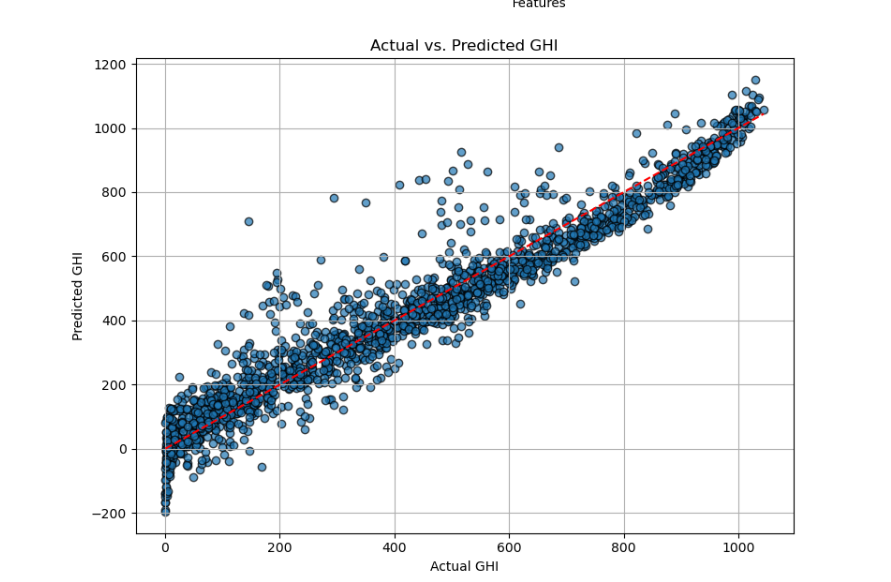
\includegraphics[width=1\linewidth]{ActualvsPredictedlinreg.png}
            \caption{Plot of actual vs predicted values for linear regression example.}
            \label{fig:enter-label}
        \end{figure}
         
    
    \label{Figure 2}
    \begin{figure}
            \centering
            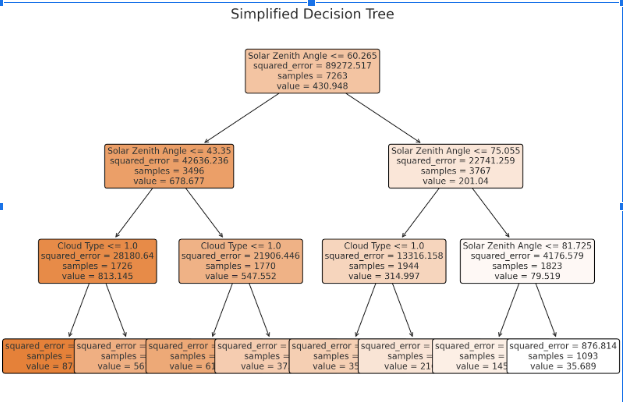
\includegraphics[width=1\linewidth]{Decisiontreevisualization.png}
            \caption{Visualization of Decision Tree.}
            \label{fig:enter-label}
        \end{figure}
         
    
    \label{Figure 3}



\subsubsection{Overall Discussion and Analysis}
 \paragraph{} Case Study 1 demonstrated the highest accuracy due to the availability of local data that captured specific climatic patterns. Next, Case Study 2 highlighted the potential of training on geographically similar regions, achieving moderate accuracy with minimal data loss. Finally, Case Study 3 revealed the most challenges, as difficulties of generalizing to San Francisco using data from distant locations were present, with higher errors and reduced robustness. Furthermore, The model's performance was strongly influenced by the geographic and climatic similarity of training data to the target location. Furthermore, neighboring regions (Case Study 2) provided sufficient overlap in climatic patterns, whereas distant regions (Case Study 3) introduced biases due to differences in solar radiation and atmospheric conditions. Additionaly, it  was observed that the stacking regressor effectively captured both linear and nonlinear dependencies, showing robustness across all cases. However, its reliance on high-quality, relevant input data limits its generalizability to regions with distinct microclimates or unique atmospheric patterns. Training on local or geographically similar data is crucial for accurate predictions, particularly for regions with unique weather phenomena. Furthermore, expanding datasets to include additional climatic variables or adaptive models could improve generalizability and reduce prediction errors.
 \subsection{Alternate Explanations and Caveats}
While the results achieved by the stacking regressor demonstrate strong predictive capabilities, several alternate explanations and caveats should be considered. First, the accuracy of the model may be partly attributed to the inherent similarities in the geographic and climatic features within the datasets used, particularly for Case Studies 1 and 2. This suggests that the high performance might not generalize to regions with more distinct climatic differences. 

Second, the limited temporal scope of the datasets (e.g., data from a specific year) may have constrained the model's ability to account for seasonal or long-term climate variations. Including multi-year data could provide a more robust understanding of solar radiation patterns.

Additionally, the reliance on specific features, such as temperature and solar zenith angle, while effective, may overlook other influential factors like pollution levels or aerosol concentrations, potentially introducing bias into the predictions. Future work should explore incorporating these additional variables to refine the model.

Finally, the computational complexity of ensemble methods like the stacking regressor, while yielding high accuracy, may limit their applicability for real-time or resource-constrained applications. Simplified models, although less accurate, could be explored for faster predictions where computational resources are limited.

By addressing these caveats and exploring alternative approaches, future iterations of the project could enhance the generalizability, robustness, and practical utility of solar radiation prediction models.

  

\section{Ethical Considerations}

Data used in this project is sourced from the National Solar Radiation Database, which is a publicly available and cost free database, ensuring compliance with the ethical standard of data accessibility. The NSRDB maintains high standards of transparency by providing open access to its datasets, along with detailed documentation on collection methodologies and potential limitations \cite{1}. This ensures that users understand the origins and reliability of the data. Additionally, the NSRDB integrates multiple sources, including ground measurement stations and satellite observations, to provide accurate and unbiased solar radiation data\cite{1}. By excluding personally identifiable information and focusing solely on environmental variables, the NSRDB safeguards privacy while enabling widespread use of its data. The database also emphasizes inclusivity by covering diverse geographic areas and climatic conditions. 


While this project strives for inclusivity, limitations in the scope of project due to time constraints may inadvertently introduce biases into machine learning models trained on this data. For instance, this project primarily utilized data from urban regions such as San Francisco, San Mateo, Berkeley, Los Angeles, and San Diego. As a result, models trained on this dataset may underperform in rural or underrepresented areas with different climatic or atmospheric conditions.
Furthermore, predictive models for solar radiation could face ethical challenges, including data bias and inequitable benefits. Models trained on data from regions like San Francisco or Los Angeles may not generalize well to underrepresented areas, limiting their applicability. Additionally, the focus on specific features, such as temperature, risks overlooking factors critical to diverse environmental contexts.

Drawing from Svoboda’s framework of non-ideal justice, predictive models should prioritize inclusivity, fairness, and transparency\cite{11}. By addressing these ethical considerations, solar radiation technologies can advance climate solutions while promoting global equity and sustainability.



Solar radiation prediction technologies have the potential to address energy inequities by supporting the development of renewable energy infrastructure. However, their implementation must be approached with caution to avoid exacerbating existing disparities. Regions with limited technological infrastructure or sparse datasets may not benefit equally from these advancements, perpetuating global energy inequities. Moreover, wealthier areas with established renewable energy projects may disproportionately benefit from these models, sidelining communities with limited access to solar infrastructure.

To mitigate these challenges, it is essential to prioritize diversity in data collection and collaborate with local communities to tailor models to their unique needs. By incorporating diverse perspectives and datasets, predictive models can better support global efforts to reduce carbon emissions and promote energy equity.


\section{Conclusion}

This project explored the development and evaluation of predictive models for solar radiation, specifically targeting Global Horizontal Irradiance (GHI). Through the use of linear regression, decision tree regression, and a stacking regressor, the study analyzed how different modeling techniques can address both linear and nonlinear dependencies in solar radiation data. The stacking regressor consistently demonstrated superior performance, highlighting the value of ensemble methods in capturing complex relationships.

The three case studies underscored the importance of data relevance and geographic similarity in model performance. Local data, as demonstrated in Case Study 1, provided the most accurate predictions, while models trained on geographically similar regions (Case Study 2) showed moderate success. However, the performance decline observed in Case Study 3, when trained on distant regions, emphasized the limitations of using non-local data.

Ethical considerations, including geographic bias, access to technology, and the societal implications of model deployment, were also addressed. These aspects highlight the necessity of equitable data practices, inclusive model design, and targeted deployment strategies to ensure that solar radiation prediction models contribute to global energy equity and sustainability.

The findings from this study reinforce the critical role of feature selection, robust model design, and diverse datasets in improving solar radiation predictions. Future work could expand on these insights by integrating deep learning techniques, real-time data inputs, and broader geographic representation. By addressing these areas, predictive models can become even more powerful tools for advancing renewable energy adoption and mitigating climate change.
\pagebreak
\newpage
\appendix

\newpage\section*{Appendix: Replication Instructions}

\subsection*{1. Software Requirements}
The following software and packages are required to replicate the project:
\begin{itemize}
    \item \textbf{Operating System:} The project is compatible with Windows, macOS, and Linux.
    \item \textbf{Python Version:} Python 3.8 or later.
    \item \textbf{Jupyter Notebook:} Install via Anaconda distribution or standalone.
    \item \textbf{Required Python Libraries:}
    \begin{itemize}
        \item pandas (version 1.3.3 or later)
        \item numpy (version 1.21.2 or later)
        \item scikit-learn (version 1.0.2 or later)
        \item matplotlib (version 3.4.3 or later)
        \item seaborn (version 0.11.2 or later)
    \end{itemize}
\end{itemize}

\subsection*{2. Installation Instructions}
\begin{enumerate}
    \item Install Python 3.8 or later from the official Python website (\url{https://www.python.org/}).
    \item Install Jupyter Notebook:
    \begin{verbatim}
    pip install notebook
    \end{verbatim}
    \item Install the required Python libraries:
    \begin{verbatim}
    pip install pandas numpy scikit-learn matplotlib seaborn
    \end{verbatim}
    \item Verify the installation by running the following command in the terminal or command prompt:
    \begin{verbatim}
    python -m pip list
    \end{verbatim}
    Ensure that the installed library versions match or exceed the required versions.
\end{enumerate}

\subsection*{3. Data Collection}
The datasets used in this project were sourced from the \textbf{National Solar Radiation Database (NSRDB)}, maintained by the National Renewable Energy Laboratory (NREL). The NSRDB provides high-resolution solar radiation data, including Global Horizontal Irradiance (GHI), Direct Normal Irradiance (DNI), and Diffuse Horizontal Irradiance (DHI), which are critical for solar energy research and predictive modeling.

\begin{itemize}
    \item \textbf{Accessing the NSRDB:} Datasets can be downloaded from the official NSRDB data viewer at \url{https://nsrdb.nrel.gov/data-viewer}.
    \item \textbf{Selection Criteria:} Data is retrieved by specifying latitude and longitude coordinates for the desired location, along with the year of interest. Each downloaded dataset includes temporal, meteorological, and atmospheric features.
    \item \textbf{Preprocessing:} Once downloaded, the datasets are preprocessed to align feature names, remove redundant columns, and handle missing values. This ensures compatibility with the modeling pipeline.
\end{itemize}

For this project, datasets were collected for the following locations: San Francisco, San Mateo, Berkeley, Los Angeles, and San Diego. All downloaded files should be saved in CSV format and placed in the project directory.

\subsection*{4. Dataset Preparation}
\begin{itemize}
    \item Place all dataset files in the same directory as the Jupyter notebook for simplified access.
    \item Ensure the datasets are preprocessed as described in the methods section to align feature names and remove unnecessary columns.
\end{itemize}

\subsection*{5. Running the Code}
\begin{enumerate}
    \item Launch Jupyter Notebook:
    \begin{verbatim}
    jupyter notebook
    \end{verbatim}
    \item Open the main project notebook file, \texttt{SolarRadiationPrediction.ipynb}.
    \item Run the notebook cells sequentially to execute the code. The notebook includes:
    \begin{itemize}
        \item Data preprocessing steps.
        \item Model training and evaluation.
        \item Visualizations and result analysis.
    \end{itemize}
    \item Outputs, including performance metrics and visualizations, will be generated in the notebook.
\end{enumerate}

\subsection*{6. Notes for Future Users}
\begin{itemize}
    \item \textbf{Compatibility:} Ensure compatibility of Python and library versions as updates may introduce breaking changes.
    \item \textbf{Reproducibility:} Use the provided requirements file to replicate the exact environment:
    \begin{verbatim}
    pip freeze > requirements.txt
    pip install -r requirements.txt
    \end{verbatim}
    \item \textbf{Dataset Updates:} If using newer datasets, ensure that they are preprocessed similarly to maintain consistency with the original analysis.
    \item \textbf{Error Handling:} Common errors, such as mismatched feature names, are documented in the notebook along with troubleshooting steps.
\end{itemize}

\subsection*{7. Additional Resources}
For further assistance, refer to the following resources:
\begin{itemize}
    \item Jupyter Notebook Documentation: \url{https://jupyter.org/}
    \item Python Package Index (PyPI): \url{https://pypi.org/}
    \item scikit-learn User Guide: \url{https://scikit-learn.org/stable/user_guide.html}
    \item National Solar Radiation Database (NSRDB): \url{https://nsrdb.nrel.gov/}
\end{itemize}




\section*{Appendix: Code Architecture Overview}

This appendix provides an overview of the code architecture, outlining the structure and organization of the project. The goal is to enable another developer to extend, debug, or enhance the project effectively. The layout below reflects the structure of the Jupyter Notebook used in this project.

\subsection*{1. Project Structure}
\begin{itemize}
    \item \textbf{Datasets:}  Each dataset is a CSV file corresponding to a specific geographic region, ensuring consistency and organization.
    \item \textbf{Notebook:} The primary analysis, modeling, and visualization are conducted in a Jupyter notebook, \texttt{SolarRadiationPrediction.ipynb}. This notebook is structured into logical sections, including data loading, preprocessing, feature exploration, model training, evaluation, and visualization.
    \item \textbf{Modules:} To streamline the workflow and promote reusability, core functionalities are implemented directly within notebook cells, as follows:
     \item\textbf{Data Preprocessing:} Handles data cleaning, feature selection, and transformations.
        \item \textbf{Model Training:} Includes model initialization, training, hyperparameter tuning, and evaluation.
        \item \textbf{Visualization:} Generates scatter plots, residual plots, correlation heatmaps, and feature importance visualizations.
        \item \textbf{Evaluation Metrics:} Calculates MAE, RMSE, and R\textsuperscript{2} scores to assess model performance.
    \end{itemize}
    \item \textbf{Results:} Output files, such as plots and evaluation summaries, can be viewed after running the cells in {SolarRadiationPrediction.ipynb}.
    \item \textbf{Dependencies:} Section 8 lists all the necessary Python packages and their versions, ensuring replicability.
\end{itemize}

    \begin{itemize}
Although my project was organized in the same directory for simplicity for the porgram to read the files, the project can be organized into the following directory and file structure. 
\begin{verbatim}
project_root/
├── datasets/
│   ├── SanFrancisco.csv
│   ├── SanMateo.csv
│   ├── Berkeley.csv
│   ├── LosAngeles.csv
│   └── SanDiego.csv
├── notebooks/
│   └── SolarRadiationPrediction.ipynb
├── results/
│   └── output_visualizations/
├── requirements.txt
└── README.md
\end{verbatim}
\subsection*{2. Execution Workflow}
\begin{enumerate}
    \item Open the Jupyter Notebook \texttt{SolarRadiationPrediction.ipynb}.
    \item Execute cells sequentially, following the outlined structure.
    \item Save outputs, including performance metrics and visualizations, in the \texttt{results/} directory.
\end{enumerate}

\subsection*{3. Jupyter Notebook Cell Layout}
The Jupyter Notebook is organized into the following sections. Note my notebook starts at line 32 as previous methods were deleted:

\subsubsection*{1. Setup}
\begin{itemize}
    \item Import necessary libraries, including pandas, numpy, scikit-learn, matplotlib, and seaborn.
    \item Load required datasets and display their structure (e.g., using \texttt{head()}).
\end{itemize}

\subsubsection*{2. Data Preprocessing}
\begin{itemize}
    \item Clean datasets by removing unnecessary columns and handling missing values.
    \item Align feature names across all datasets to ensure consistency.
    \item Generate and visualize a correlation matrix to identify relationships between features and the target variable (GHI).
    \item Split data into training and testing sets with an 80/20 split.
\end{itemize}

\subsubsection*{3. Model Training}
\begin{itemize}
    \item Train and evaluate a Linear Regression model.
    \item Train and tune a Decision Tree Regressor, including hyperparameter tuning using GridSearchCV.
    \item Train a Stacking Regressor combining the Linear Regression and Decision Tree models.
\end{itemize}

\subsubsection*{4. Evaluation Metrics}
\begin{itemize}
    \item Compute performance metrics for each model:
    \begin{itemize}
        \item Mean Absolute Error (MAE).
        \item Root Mean Squared Error (RMSE).
        \item R-squared (\( R^2 \)).
        \item Predicted \( R^2 \) using cross-validation.
    \end{itemize}
    \item Display metrics in tabular form for comparison.
\end{itemize}

\subsubsection*{5. Visualization}
\begin{itemize}
    \item Generate scatter plots comparing actual vs. predicted GHI values for each model.
    \item Create residual plots to analyze prediction errors.
    \item Plot feature importance for the Decision Tree model.
    \item Visualize cross-validation scores for the Stacking Regressor.
\end{itemize}

\subsubsection*{6. Case Studies}
\begin{itemize}
    \item Analyze model performance on individual case studies, including:
    \begin{itemize}
        \item Localized predictions using San Francisco data.
        \item Predictions for San Francisco using models trained on combined San Mateo and Berkeley data.
        \item Predictions for San Francisco using models trained on combined Los Angeles and San Diego data.
    \end{itemize}
    \item Discuss insights and implications from each case study.
\end{itemize}

\subsubsection*{7. Analysis}
\begin{itemize}
    \item Summarize findings from the models and case studies.
    \item Highlight strengths, limitations, and potential improvements.
\end{itemize}



\subsection*{4. Extensibility and Debugging}
\begin{itemize}
    \item \textbf{Debugging:} Inline comments and logical grouping of cells make it easier to identify and fix issues.
    \item \textbf{Incorporate New Data:} Add datasets for additional geographic regions in the \texttt{datasets/} directory and update the preprocessing and training pipeline to include these files.
    \item \textbf{Add New Models:} Include additional machine learning algorithms (e.g., Random Forests, Gradient Boosting) by appending new cells for model implementation and evaluation.
    \item \textbf{Enhance Visualizations:} Modify visualization cells to include interactive plots or additional performance metrics using libraries such as Plotly.
    \item \textbf{Real-Time Prediction:} Develop an API or integration for real-time prediction by exporting the trained models and using them in a live environment.
\end{itemize}

This layout ensures that the project is accessible for replication, extensibility, and debugging, enabling effective collaboration and adaptation.



\end{itemize}

\subsection{Code Architecture Diagram}
The following diagram illustrates the organization of the project:

\begin{figure}[h]
    \centering
    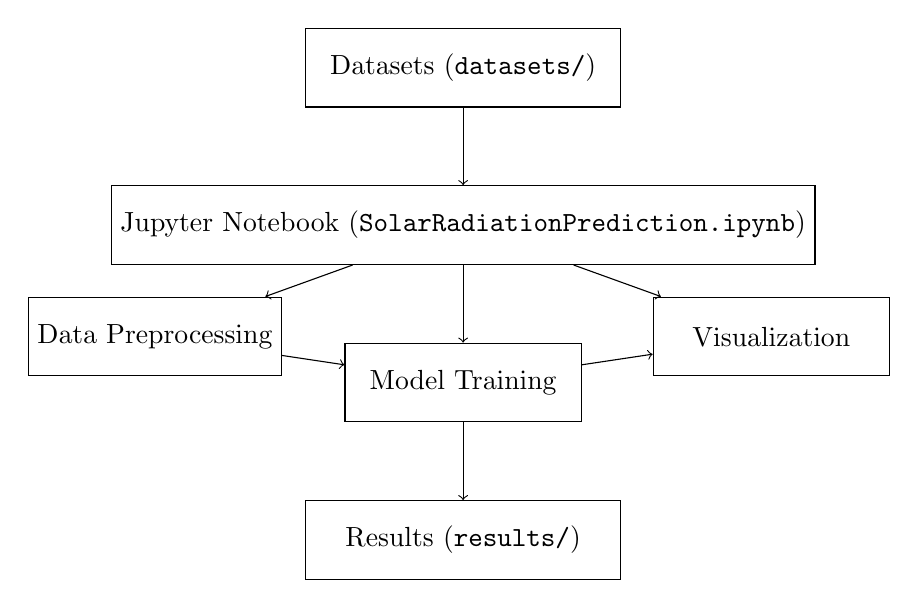
\begin{tikzpicture}[node distance=2cm]
        % Define nodes
        \node (datasets) [rectangle, draw, text centered, minimum width=4cm, minimum height=1cm] {Datasets (\texttt{datasets/})};
        \node (notebook) [rectangle, draw, below of=datasets, text centered, minimum width=6cm, minimum height=1cm] {Jupyter Notebook (\texttt{SolarRadiationPrediction.ipynb})};
        \node (preprocessing) [rectangle, draw, below left of=notebook, text centered, minimum width=3cm, minimum height=1cm, xshift=-2.5cm] {Data Preprocessing};
        \node (training) [rectangle, draw, below of=notebook, text centered, minimum width=3cm, minimum height=1cm] {Model Training};
        \node (visualization) [rectangle, draw, below right of=notebook, text centered, minimum width=3cm, minimum height=1cm, xshift=2.5cm] {Visualization};
        \node (results) [rectangle, draw, below of=training, text centered, minimum width=4cm, minimum height=1cm] {Results (\texttt{results/})};

        % Draw arrows
        \draw[->] (datasets) -- (notebook);
        \draw[->] (notebook) -- (preprocessing);
        \draw[->] (notebook) -- (training);
        \draw[->] (notebook) -- (visualization);
        \draw[->] (preprocessing) -- (training);
        \draw[->] (training) -- (visualization);
        \draw[->] (training) -- (results);
    \end{tikzpicture}
    \caption{Code Architecture Overview}
    \label{fig:code_architecture}
\end{figure}

\subsection{5. Justification of Design}
This architecture promotes:
\begin{itemize}
    \item \textbf{Modularity:} Functions and operations are organized within various cells of the notebook, making the workflow easy to follow and debug.
    \item \textbf{Reusability:} Key processes, such as data preprocessing and evaluation metrics, can be reused across different datasets or models.
    \item \textbf{Scalability:} The structure supports  integration of additional datasets, features, or models without major architectural changes.
    \item \textbf{Transparency:} The Jupyter notebook provides a clear narrative of the workflow, ensuring replicability and ease of understanding for new contributors.
\end{itemize}
\subsection*{8. Requirements File}
Below lists all the necessary Python packages and their versions, ensuring replicability.
\begin{verbatim}
pandas==1.3.3
numpy==1.21.2
scikit-learn==1.0.2
matplotlib==3.4.3
seaborn==0.11.2
notebook==6.4.3
\end{verbatim}










\newpage
\begin{thebibliography}{200}

\bibitem{nsrdb} National Renewable Energy Laboratory. (n.d.). Retrieved from \url{https://nsrdb.nrel.gov/data-viewer}.
\bibitem{nasa_climate_effects} NASA. (n.d.). Climate Change Effects. Retrieved from \url{https://science.nasa.gov/climate-change/effects/}.

\bibitem{regression_models} Solar Power Prediction using Regression Models. Retrieved from \url{https://www.researchgate.net/publication/366613171_Solar_Power_Prediction_using_Regression_Models}.

\bibitem{iopscience} IOPscience. (n.d.-b). Retrieved from \url{https://iopscience.iop.org/article/10.1088/1755-1315/830/1/012080/pdf} and \url{https://www.azocleantech.com/article.aspx?ArticleID=1727}.

\bibitem{ensemble_models} Sehrawat, N., et al. (2023). Solar irradiance forecasting models using machine learning techniques and digital twin: A case study with comparison. Retrieved from \url{https://www.sciencedirect.com/science/article/pii/S2666603023000064}.

\bibitem{feature_selection} Gupta, R., Salcedo-Sanz, S., et al. (2024). Composition of feature selection techniques for improving the global horizontal irradiance estimation via machine learning models. Retrieved from \url{https://www.sciencedirect.com/science/article/abs/pii/S245190492400012X}.

\bibitem{ghi_topic} Global Horizontal Irradiance. (n.d.). Retrieved from \url{https://www.sciencedirect.com/topics/engineering/global-horizontal-irradiance}.

\bibitem{africa_hybrid_models} Kassem, Y., Camur, H., Adamu, M. T., Chikowero, T., & Apreala, T. Prediction of solar irradiation in Africa using linear-nonlinear hybrid models. Retrieved from \url{https://www.etasr.com/index.php/ETASR/article/view/6131}.

\bibitem{site_adaptation} Narvaez, G., Giraldo, L. F., Bressan, M., & Pantoja, A. (2023). Machine learning for site-adaptation and Solar Radiation Forecasting. Retrieved from \url{https://hal.science/hal-04070113}.

\bibitem{geospatial_ethics} Geospatial Data. Ethics & Applications of Geospatial Technologies. LibGuides at University of Texas at Austin. Retrieved from \url{https://guides.lib.utexas.edu/grg356t}. Accessed 22 Apr. 2024.

\bibitem{geodata_privacy} Privacy Challenges in Geodata and Open Data. Retrieved from \url{https://rgs-ibg.onlinelibrary.wiley.com/doi/full/10.1111/area.12888}. Accessed 22 Apr. 2024.

\bibitem{thin_films} Nkuissi, H. J. T., Konan, F. K., Hartiti, B., & Ndjaka, J.-M. (2020). Toxic materials used in thin film photovoltaics and their impacts on environment. Retrieved from \url{https://www.intechopen.com/chapters/68288}.

\bibitem{toxic_solar} Shellenberger, M. (2022). Dark Side to Solar? More Reports Tie Panel Production to Toxic Pollution. Forbes. Retrieved from \url{https://www.forbes.com/sites/michaelshellenberger/2021/06/21/why-everything-they-said-about-solar---including-that-its-clean-and-cheap---was-wrong/?sh=7f50ab595fe5}.

\bibitem{human_rights_solar} Solar vs Human Rights: Hidden Ethical Issues with Solar Panels. (n.d.). Retrieved from \url{https://www.frdm.co/blogs/solar-vs-human-rights}.

\bibitem{energy_proceedings} Energy Proceedings. (n.d.). Machine learning models for solar irradiance prediction. Retrieved from \url{https://www.energy-proceedings.org/wp-content/uploads/icae2021/1642315686.pdf}.
\bibitem{ethics_climate} Svoboda, T. (n.d.). The ethics of climate engineering: Solar radiation management and non-ideal justice. Retrieved from \url{https://ndpr.nd.edu/reviews/the-ethics-of-climate-engineering-solar-radiation-management-and-non-ideal-justice/}.
\bibitem{Boutahir2022} Boutahir, M. K., Farhaoui, Y., Azrour, M., Zeroual, I., & El Allaoui, A. (2022). Effect of feature selection on the prediction of direct normal irradiance. \textit{Big Data Mining and Analytics, 5}(4), 309--317. \url{https://doi.org/10.26599/BDMA.2022.9020003}

\bibitem{Kumari2021} Kumari, P., & Toshniwal, D. (2021). Machine learning techniques for hourly global horizontal irradiance prediction: A case study for smart cities of India. \textit{Energy Proceedings, 18}, 69. \url{https://www.energy-proceedings.org/wp-content/uploads/icae2021/1642315686.pdf}

\bibitem{Khalifa2022} Khalifa, B. M., Farhaoui, Y., Azrour, M., Zeroual, I., & El Allaoui, A. (2022). Exploring and forecasting solar radiation with machine learning models. \textit{Energy Reports}. Retrieved from \url{https://www.energy-reports.org}
\bibitem{AnalyticsVidhya2019} Analytics Vidhya. (2019). 11 Important Model Evaluation Metrics. Retrieved from \url{https://www.analyticsvidhya.com/blog/2019/08/11-important-model-evaluation-error-metrics/}

\bibitem{ScikitLearnTree} Scikit-learn. (n.d.). Tree regression example. Retrieved from \url{https://scikit-learn.org/1.5/auto_examples/tree/plot_tree_regression.html}

\bibitem{AnalyticsVidhya2020} Analytics Vidhya. (2020). Improve Predictive Model Score Using Stacking Regressor. Retrieved from \url{https://www.analyticsvidhya.com/blog/2020/12/improve-predictive-model-score-stacking-regressor/}


\end{thebibliography}





\printbibliography
\end{document}

